\section{Brain-Computer Interface}
Due to the broad spectrum of cognitive disorders caused by neurological degradation due to old age or disease, cognitive-aids can be classified in many different categories. One major cognitive-aid category is Brain-Computer Interfaces (BCIs). In a broad sense, BCIs are used to infer volitional thought processes of their users and convert them into accessible signals. These signals can be used by an external device or other humans in the case of communications. To this end, devices record brain activity and generally apply some post-processing to generate a signal useful for another application. BCIs can either be noninvasive or invasive. Noninvasive devices typically use EEG sensors while invasive devices incorporate ECoG and ____ sensors. 

--Invasive BCIs and Non-Invasive BCIs reorganize the paragraphs.

\subsection{Brain-Computer Interface}
\begin{figure}[t]
    \centering
    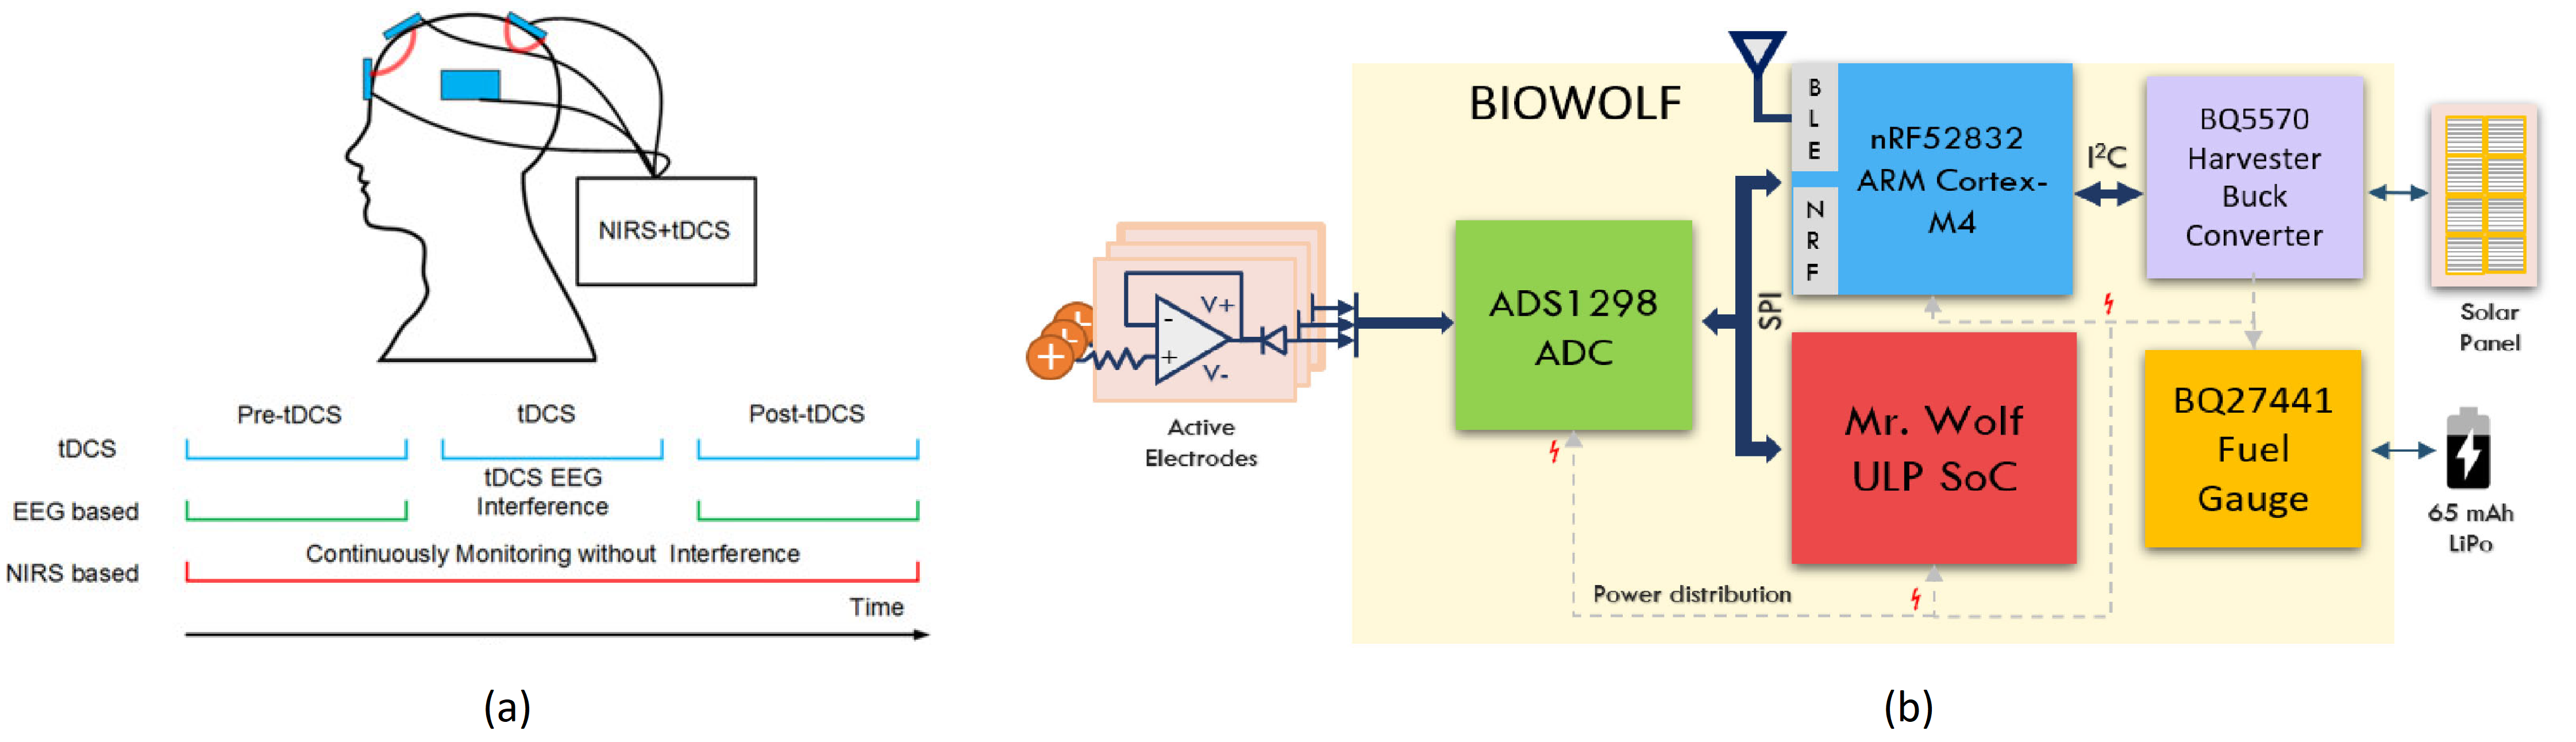
\includegraphics[width=\textwidth]{Figure/CognitiveAid/BCIcollage3}
    \caption{Brain-machine interface devices. (a) Illustration given in \textcite{miao_cmos-based_2018} of NIRS and tDCS systems integrated with different configurations that can be applied due to lack of cross-coupling. (b) Illustration given in \textcite{kartsch_biowolf_2019} of BioWolf system block diagram.}
    \label{fig:BCICollage}
\end{figure}
\textcite{lin_review_2010} characterizes 32 BCI devices based on seven design attributes of which four are described here. The first attribute, transmission media, looks at whether the system is wired or wireless. The next attribute, target users, infers the system application based on the study that the authors presented in their paper. If the study was conducted with healthy participants, it can be inferred that the system is for general commercial use. On the other hand, if the study participants have a specific disability then the that subgroup is concluded as the target users. The third attribute, sensor placement, refers to whether invasive ECoG electrodes or noninvasive EEG electrodes are used. Lastly, the neurological phenomenon attribute references the signal trend or phenomenon that is `detected' in post-processing to trigger the next stage. For example, one of the reviewed BCI systems by \textcite{ming_cheng_design_2002} uses steady-state visual evoked potentials (SSVEP) to identify user button selection on a virtual telephone keypad. In this case, the neurological phenomenon that triggers the keypad dialing is the SSVEP.

\textcite{miao_cmos-based_2018} presents a noninvasive BCI that uses transcranial direct-current stimulation (tDCS) with dynamic dosage adjustment. tDCS is a noninvasive approach that uses electrodes connected to the skull for stimulation. In prior work \parencite{roh_wearable_2014}, devices using tDCS ran into dynamic stimulation adjustment issues because of electroencephalogram (EEG)-based closed-loop techniques coupled with the electrical stimulation mechanism. The proposed device in \textcite{miao_cmos-based_2018} uses frequency-domain near-infrared spectroscopy (fdNIRS) that side-steps the issue of electrical coupling by using optical recording as part of the feedback mechanism. Sensing of cerebral hemodynamics is done with signal processing techniques applied on a fdNIRS signal captured by a simple avalanche photodiode. 

\textcite{kartsch_biowolf_2019} proposes a BCI device that tackles a primary limiting factor in the wide adoption of BCIs, which is inadequate battery life and processing power. An improvement in one of these areas results in a reduction in the other. \textcite{kartsch_biowolf_2019} proposes a novel parallel digital signal processing (DSP) chip and microcontroller architecture that increases the processing power while simultaneously keeping system power consumption low. The system directly converts brain signals collected by active electrodes into digital signals via a commercial analog-to-digital converter. The resulting signal is fed into a parallel ultra-low-power system-on-a-chip (SoC) designed by the authors in \textcite{pullini_mr_2018} dubbed Mr.Wolf. The Mr.Wolf SoC uses nine RISC-V processors arranged in parallel optimized with additional hardware to implement DSP algorithms. The resulting non-invasive system along with a solar energy harvester and a commercial low-power RF communication chip were tested on five healthy subjects. The results showed that the device battery life was up to 38 hours.

\textcite{zhou_hybrid_2020} explores ways to improve the performance of BCIs by combining  EOG- and SSVEP-based eye trackers. SSVEP-based eye trackers are asynchronous BCIs that have a major drawback of not being able to distinguish between an idle and a control state. Eyeblink detection in EOG sensory can overcome the mentioned challenge of SSVEP. In the combined system, while SSVEP signals determine whether the user's eye focuses on the control button, the EOG sensory detects the user's eye blinks. The only case that issues a command in the control state is when the user pays attention to the command button and blinks an eye. This method effectively reduces the false-positive rate (FPR). While wearable EEG electrodes on the user's head record the SSVEP signals, a single electrode on the forehead monitors the EOG signal along with a reference electrode on the right mastoid. To test the command accuracy and FPR,  ten subjects with healthy vision participated in free spelling experiments. The free spelling test requires each subject to select 48 predefined characters and then remain in the idle state for 10 minutes. The achieved performance of the proposed hybrid BCI is 95.42\% $\pm$ 2.15\% accuracy and 0.80\% $\pm$ 0.75\% FPR. Testing with the same subjects using conventional SSVEP based BCIs resulted in a slightly worse accuracy of 94.58\% $\pm$ 7.16\% and a higher FPR of 12.77\% $\pm$ 8.55\% which shows the positive impact of the eye trackers used in the proposed BCI. 

\textcite{deng_bayesian_2020} explores the applications of SSVEP further by taking advantage of another SSVEP eye tracking application. SSVEP develops in the visual cortex when a subject focuses on a flickering visual stimulus \parencite{nakanishi_high-speed_2014}. SSVEP signals are extracted from EEG signals and utilized to issue a control command of the environment. \textcite{deng_bayesian_2020} presents a Bayesian-shared-control human-machine interface to control a smart wheelchair using this form of eye tracking. The system integrates a stimuli module consisting of 4 LEDs where each LED represents one command. The wheelchair direction control options are move forward, slow down, turn left, and turn right. The wheelchair turn angle choices range from 0$^{\circ}$ to  90$^{\circ}$ in 30$^{\circ}$ increments. As the stimulus paradigm is two-layer, the user needs to command a direction before an angle command. When the user's eye focuses on either LED, the SSVEP signals will respond, and the related control command will be issued. The experiments were performed with eleven healthy subjects to test the wheelchair motion controls'  accuracy through the proposed BSC-HMI. For the online test, each subject was required to control the wheelchair passing along a particular route five times. The average statistical reliability of BSC-HMI was 71.82\%.  A deep learning approach is planned to be employed to decode EEG signals and apply various stimulus paradigms as the next step of this work to reduce the latency.

%%%%%%%%%%%%%%%%%%%%%%%%%%%%%%%%%%%%%%%%%%%%%%%%%%%%%%%%%%%%%%%%% SECTION REMOVED %%%%%%%%%%%%%%%%%%%%%%%%%%%%%%%%%%%%%%

% \subsection{General Cognitive Aids}
% \begin{figure}[t]
%     \centering
%     \includegraphics[width=\textwidth]{Figure/CognitiveAid/GCACollage3}
%     \caption{General cognitive aids. (a) Illustration given in \textcite{jia_mm-sized_2020} of optical and electrical stimulation headstage and implanted device in a rat. (b) Microscopic photograph given in \textcite{yamakawa_implantable_2019} of the fabricated probe head with ECoG, temperature, and photodiode sensors}
%     \label{fig:GCACollage}
% \end{figure}
% BCI devices are not the only form of cognitive aids. There are a plethora of devices that perform functions such as invasive and non-invasive measurement of signals correlated with brain activity as well as both optical and electrical stimulation of the brain. 
% %But, they are not meant to act as BCIs. 
% For instance, \textcite{yamakawa_implantable_2019} presents an implantable flexible strip device designed to measure brain temperature, electrical activity, and oxygenation levels during surgery. Brain temperature is measured using a simple negative temperature coefficient thermistor. Six-channel platinum ECoG electrodes record the electrical activity. The oxygenation levels are determined by shining a light on the tissue and analyzing the change in amplitude and phase of the reflected signal. Since the flexible string is only used during surgery, the system lacks a wireless data transfer module. However, this device shows the promise of integrating three relevant sensing modalities; therefore, it could lead to future research in the design of wireless, permanently implanted devices similar to this one. 

% \textcite{jia_mm-sized_2020} proposes a monitoring system, where the sensing portion is implanted and the data is wirelessly transmitted to an external source. The system can stimulate the brain by both electrical and optical stimulation mechanisms and also close the loop with neural recording. Despite being less power efficient, the advantage of optical stimulation is that it is cell type-specific. As a way to benefit from the best of both stimulation modalities, \textcite{jia_mm-sized_2020} presents a device that offers 16-channel optical and 4-channel electrical stimulation. The proposed device consists of a headstage and one or more small implantable modules, called free-floating wireless implantable optoelectric stimulators (FF-WIOS2). The headstage communicates via low-energy Bluetooth to external devices as well as by inductive link to one or more FF-WIOS2 using on-off keying. Each FF-WIOS2 device has electrodes for electrical stimulation and uLEDs for optical stimulation. 

% Moving away from monitoring different brain signals, there is also a whole field dedicated to stimulation. Stimulation of the brain is a proven treatment for some neurological disorders that affect movements. \textcite{amon_systems_2017} reviews and compares many commercially available Deep Brain Stimulators (DBSs) produced mainly by Boston Scientific (B), Medtronic (M), and St. Jude (S). Reviews are based on a variety of technical considerations including electrical source, number of implantable pulse generators (IPGs), electrode design, polarity, and electrical stimulation signal. According to the review, B devices offered current source stimulation to avoid issues with impedance changes that affect stimulation current. B devices also have more than one IPG to enable stimulation of each hemisphere of the brain separately if desired. Segmented eight electrode design with multi-polar configurations was also used by B devices. Finally, many stimulation configurations offered by B devices allow the treatment of different symptoms and limit unwanted side effects of stimulation outside the localized region. S devices also provide the same features as the B devices except for not being able to set different amplitude levels for each contact during stimulation. M devices varied mainly in electrode design, where their systems were equipped with classic unipolar ring contact electrodes. They also shared the S device characteristic of being designed with a single current source in contrast to B devices.

%%%%%%%%%%%%%%%%%%%%%%%%%%%%%%%%%%%%%%%%%%%%%%%%%%%%%%%%%%%%%%%%%%%%%%%%%%%%%%%%%%%%%%%%%%%%%%%%%%%%%%%%%%%%%%%%%%%%%%%%

\subsection{Sensors In Use}
This section will highlight sensors that are distinct to the cognitive aid field. However, it should be noted that there are many redundant sensors in use with cognitive aids that are not highlighted since they have been discussed in previous sections.

% \subsubsection{Platinum ECoG Electrodes}
% Platinum electrodes are among metals that do not participate in the sensing chemical reaction. As a result, they are more stable and well suited for amperometric (i.e., current) sensing \parencite{ida_sensors_2013}. These types of sensors are referred to as ``polarizable'' electrodes. In \textcite{yamakawa_implantable_2019}, platinum electrodes are used to measure ECoG signals during brain surgery.

% \subsubsection{NTC Thermistors}
% Thermistors are generally made of a semiconducting material that has a high temperature coefficient. The material resistance changes with respect to temperature in a non-linear manner \parencite{ida_sensors_2013}. The proportionality of resistance to temperature can either be direct or inverse, depending on the sign of the temperature coefficient, i.e. positive temperature coefficient (PTC) or negative temperature coefficient (NTC). In \textcite{yamakawa_implantable_2019}, an NTC thermistor is used to measure the surface temperature of the cerebral cortex during brain surgery. 

% \subsubsection{Avalanche Photodiodes}
% Avalanche photodiodes are a subcategory of photodiodes that take advantage of the avalanche effect to act as photomultiplier sensors \textcite{ida_sensors_2013}. As a result, these photodiodes are more sensitive than photoconductive mode diodes, more advantageous in certain applications. For example, in \textcite{miao_cmos-based_2018} the system requires the detection of photocurrents as small as 10 nA. For this example, avalanche photodiodes are used due to their high sensitivity.  


%%%%% These are from Yifei's section. Aatreya, these are more relavant to your section. Could you please blend in?

%\subsubsection{Electrode}

%Electrodes are used for EEG and EOG signals detection. As GKP and SSVEP levels are potential alteration of the EEG signals, EEG active %electrodes can effectively detect GKP and SSVEP levels. 
%A commercial biopotential measurement system with active electrodes, Biosemi ActiveTwo, is used in (Nam et al., 2016) for SSVEP potential level %detection. Biosemi ActiveTwo is capable of recording from up to 264 electrodes with a maximum 16 kHz sampling rate. This study uses 33 %electrodes with a sampling rate of 2048 Hz. The user wearing a set of electrodes on Biosemi ActiveTwo could control a powered wheelchair %through the proposed TDS.